\documentclass[mathserif]{beamer}
\usepackage{appendixnumberbeamer}
\usepackage[nofirafonts]{beamerthemefocus}
\usepackage{amsmath}
\usepackage{graphicx}
\usepackage{natbib}
\usepackage{floatrow}
\usepackage{booktabs}
\usepackage{multirow}

\usepackage{xeCJK}
\setCJKmainfont{Iansui094-Regular}

\title{檢視中國債務陷阱\\Examining the Chinese Debt-Trap Diplomacy}
\author{陳家威\\{\small R10323045}}
\date{112年7月12日}

\begin{document}

    \begin{frame}

        \maketitle

    \end{frame}

    \section{Debt Trap}

    \begin{frame}
        \frametitle{A port lent for 99 years, and the emptiest ariport}
        \begin{columns}
            \begin{column}{0.48\textwidth}
                    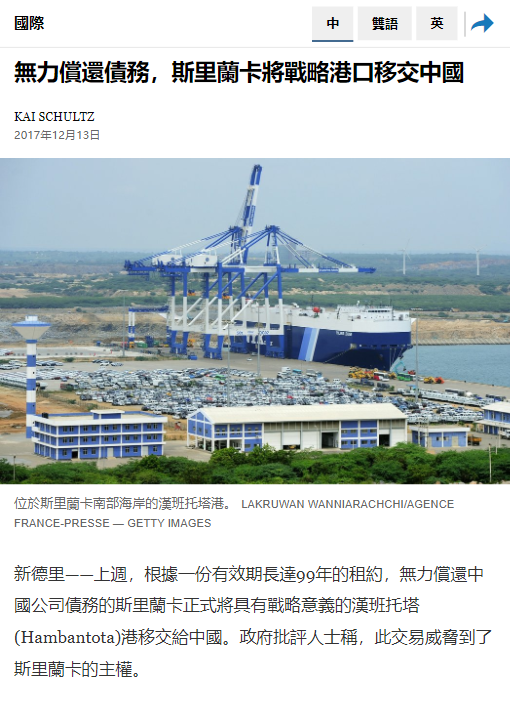
\includegraphics[width = \textwidth]{fig/Hambontota_news.png}
                    \footnotesize {Source: NYTimes}
            \end{column}%
            \pause%
            \begin{column}{0.48\textwidth}
                    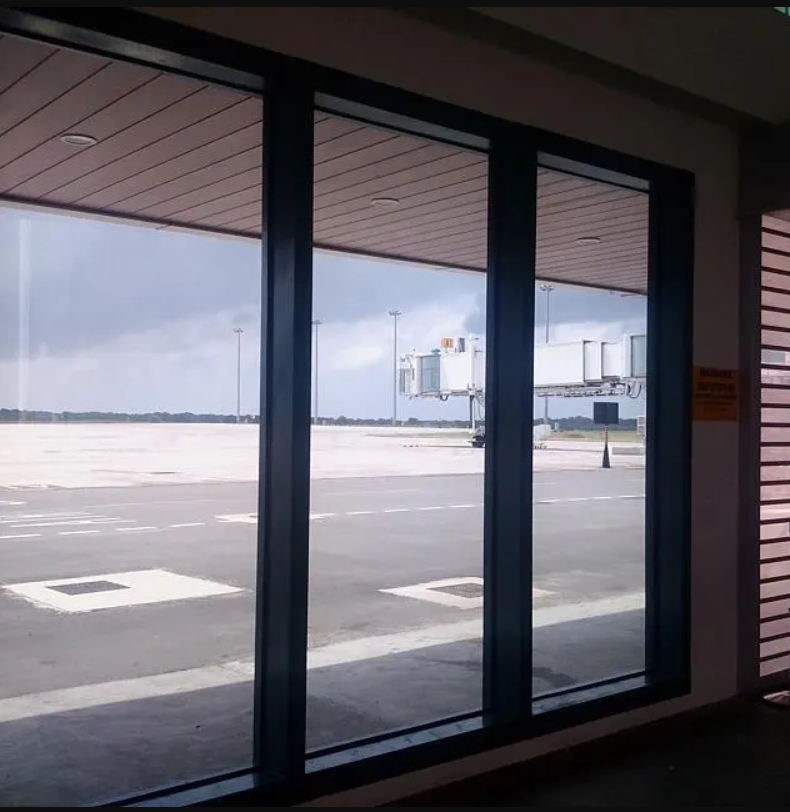
\includegraphics[width = \textwidth]{fig/empty_airport.png}
                    \footnotesize {Source:Forbes}
            \end{column}
        \end{columns}
    \end{frame}

    \begin{frame}
        \frametitle{A Crucial Role in BRI}
        \includegraphics<1>[width = \textwidth]{fig/BRI.png}%
    \end{frame}

    \begin{frame}
        \frametitle{Dept-Trap Diplomacy}
            First mentioned in \citet{Chellaney_2017}
            \begin{block}{Debt-trap Diplomacy}
               The creditor country is said to extend excessive credit to a debtor country with the intention of extracting economic or political concessions when the debtor country becomes unable to meet its repayment obligations.
            \end{block}
    \end{frame}

    \begin{frame}
        \frametitle{Debt to China}
            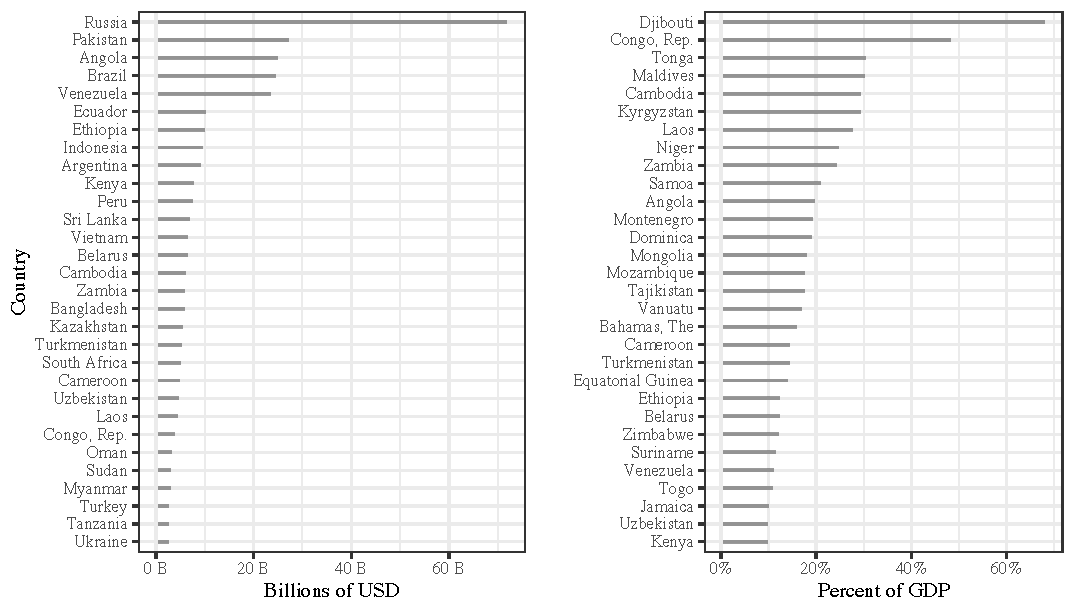
\includegraphics[width = \textwidth]{fig/debt-level-by-country.pdf}
    \end{frame}

    \begin{frame}
        \frametitle{Sri Lanka Project List}
        Hambantota Port
        \begin{itemize}
            \item Initiated: 2007
            \item 2008: Phase I, \$307 million from Chinese Exim Bank, 6\% rate
            \item 2012: Phase II, \$304 million
            \item 2017: 99-year lease, 70\% sale to China Merchant Port
        \end{itemize}
        \vfill
        Mattala Rajapaksa International Airport
        \begin{itemize}
            \item 2009: \$181 million from Chinese Exim Bank, 2\% rate
            \item 2013: Open
            \item 2014: 21,000 passengers only
            \item ``The world's emptiest airport'
        \end{itemize}
        \vfill
        Road Projects
        \begin{itemize}
            \item 2009: \$1.14 billion Colombo-Katunayake Expressway (CKE)
            \item 2010\&2011: 1.51\%
            \item 2014: \$1.99 on road construction and improvement
        \end{itemize}
    \end{frame}

    \begin{frame}
        \frametitle{Zambia Project List}
        Hydropower Station
        \begin{itemize}
            \item Initiated: 2015
            \item 2017: \$1.5 billion from Chinese Exim Bank and Industrial and Commercial Bank of China
        \end{itemize}
        Telecommunication
        \begin{itemize}
            \item Zambia National Broadcasting (ZNBC) and StarTimes (四达时代) joint revenue - Topstar Communications Company.
            \item StarTimes own 60\%
            \item 2017: \$280 million from Exim
            \item The first interest payment: \$2.3 million due in July 2017 was not paid on time
            \item StarTimes has thus taken over some of ZNBC activities, and will manage Topstar until the loan has been paid in full\citep{ofstad2019zambia}.
        \end{itemize}
    \end{frame}

    \begin{frame}[label = {sri_ts}]
        \frametitle{China's Lending to Sri Lanka}
        \begin{center}
            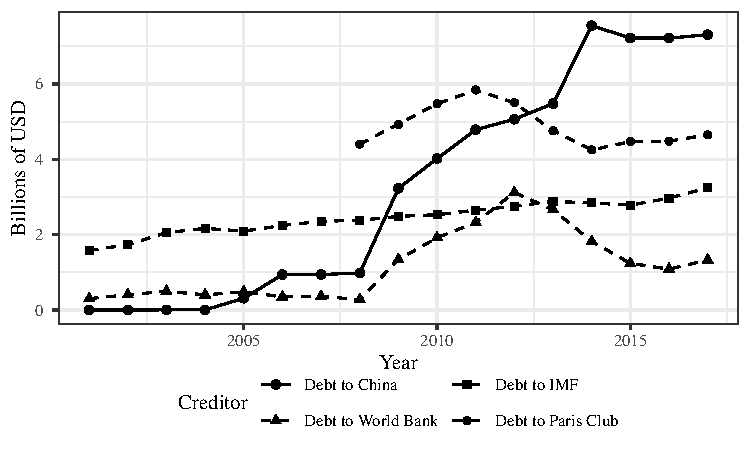
\includegraphics[width = 0.8\textwidth]{fig/ALL/Sri Lanka_debt_source.pdf}\\
            \small \hyperlink{sri_ds<2>}{Source: }\citet*{Horn-Reinhart-Trebesch-21}
        \end{center}
    \end{frame}

    \begin{frame}[label = {pak_ts}]
        \frametitle{China's Lending to Zambia}
        \begin{center}
            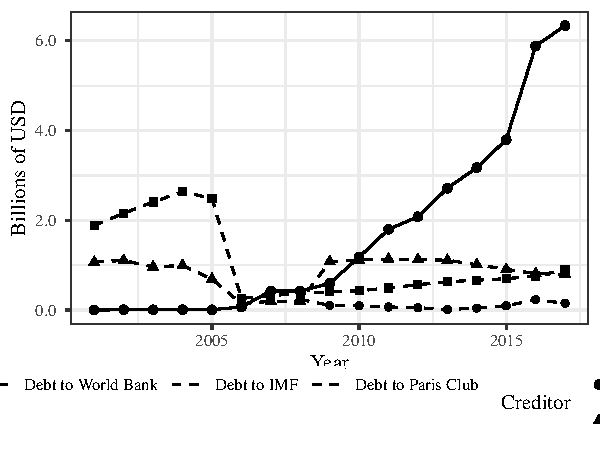
\includegraphics[width = 0.8\textwidth]{fig/ALL/Zambia_debt_source.pdf}\\
            \small \hyperlink{pak_ds}{Source: }\citet*{Horn-Reinhart-Trebesch-21}
        \end{center}
    \end{frame}

    \begin{frame}
        \frametitle{Our question: Did China Lend too much?}
            \begin{block}{Debt-trap Diplomacy}
               The creditor country is said to extend excessive credit to a debtor country with the intention of extracting economic or political concessions when the debtor country \textbf{becomes unable to meet its repayment obligations}.
            \end{block}
            \pause
            \vfill
            Key feature here is to model ``default``.
    \end{frame}

    \begin{frame}
        \frametitle{Past Studies on the Narative}
            Most studies put stress solely on the dept-to-gdp ratio, but not emphasizing default decision
            \vfill
            \pause
            \begin{itemize}
            \item \citet{Hurley19-8-debt-trap}:
            Evaluate the debt sustainability in
BRI countries by examining their dept-to-GDP ratio versus their share of China’s debt
                \begin{itemize}
                    \item Following the threshold of 50-6\% rising debt-to-GDP ratio constructed by \citet{Chudik-15}, they identify eight countries that are particularly risky.
                    \item threshold is cross-country panel threshold output growth model
                \end{itemize}
            \pause
            \item \citet{Bandiera-Vasileios-BRI-debt} analyze the growth effects of BRI investment and estimates the potential increase in debt vulnerabilities for certain countries through a model-based growth projection.
            \end{itemize}
    \end{frame}
    \section{Model}
    \begin{frame}
        \frametitle{Model Setting}

        \begin{itemize}
            \item \citet{Na-18}
            \item Decentralized version of Eaton-Gersovitz model
            \item Tradable vs Nontradable goods
            \item Household, Firm, Government, Foreign lender
        \end{itemize}

    \end{frame}

    \begin{frame}
        \frametitle{Household}
        \begin{itemize}
            \item Maximize
                \begin{equation}
                    E_0 \sum_{t=0}^\infty \beta^t U(c_t)
                \end{equation}
            \item Utility function
                \begin{equation}
                    U(c_t) = \frac{c_t^{1-\sigma} - 1}{1 - \sigma}
                \end{equation}
            \item Aggregation function for consumption
                \begin{equation}
                    \label{eq:aggregator-function}
                    c_t = A(c^T_t, c^N_t) =
                        \left[ a \left( c^T_t \right)^{1- \frac{1}{\xi}} +
                            (1 - a) \left( c^N_t \right)^{1- \frac{1}{\xi}}
                        \right]^{\frac{1}{1 - \frac{1}{\xi}}}
                \end{equation}
            \item Budget constraint
                \begin{equation}
                    \label{eq:bc}
                    P^T_t c^T_t + P^N_t c^N_t + P^T_t d_t =
                    P^T_t \tilde{y}^T_t + W_t h_t + (1- \tau^d_t)P^T_t q^d_t d_{t+1} + F_t + \Phi_t
                \end{equation}
            \item Working hours
                \begin{equation}
                    \label{eq:h-constraint}
                    h_t \le \bar{h}
                \end{equation}
        \end{itemize}
    \end{frame}

    \begin{frame}
        \frametitle{HH F.O.C}
        Notation:
$p_t \equiv \frac{P^N_t}{P^T_t}$, $w_t = \frac{W_t}{P^T_t}$, $f_t = \frac{F_t}{P^T_t}$, and $\phi_t = \frac{\Phi_t}{P^T_t}$
            \begin{subequations}
                \begin{align}
                    p_t &= \frac{A_2(c_t^T, c_t^N)}{A_1(c_t^t, c_t^N)} \label{eq:FOC-HH-1} \\
                    \lambda_t &= U'(c_t)A_1(c_t^T, c_t^N)\\
                    (1-\tau_t^d)q_t^d \lambda_t &= \beta E_t \lambda_{t+1}
                \end{align}
            \end{subequations}
    \end{frame}

    \begin{frame}
        \frametitle{Firms}
            \begin{itemize}
                \item Technology
                    \begin{equation}
                        \label{eq:production}
                        y^N_t = F(h_t)
                    \end{equation}
                \item Profit
                    \begin{equation}
                        \label{eq:profit}
                        \Phi_t(h_t) = P^N_t F(h_t) - W_t h_t
                    \end{equation}
                \item F.O.C
                    \begin{equation}
                        \label{eq:firm-FOC}
                        p_t F'(h_t) = w_t
                    \end{equation}
            \end{itemize}
    \end{frame}

    \begin{frame}
        \frametitle{Downward Wage Rigidity}

        \begin{equation}
            W_t \ge \gamma W_{t-1}, \qquad \gamma > 0
        \end{equation}
        This implies that the growth rate
        $\frac{W_{t} - W_{t-1}}{W_{t-1}} \ge \gamma - 1$

        \vfill
        Slackness condition

        \begin{equation}
            \label{eq:wage-rigid}
            (\bar{h} - h_t)(W_t - \gamma W_{t-1}) = 0
        \end{equation}
    \end{frame}

    \begin{frame}
        \frametitle{Government}

        Government decides to default of not for the economy
        \begin{itemize}
            \item If repay $(I=1)$: able to lend in $t+1$, or $d_{t+1} > 0$
            \item If default $(I=0)$: excluded from international credit market, $d_{t+1} = 0$
        \end{itemize}
        Written as slackness condition
        \begin{equation}
            \label{eq:gov-next-debt}
            (1 - I_t)d_{t+1} = 0
        \end{equation}
        \vfill
        Government returns tax to household via lump-sum transfer

        \begin{equation}
            \label{eq:gov-budget}
            f_t = \tau_t^d q_t^d d_{t+1} + (1-I_t)d_t
        \end{equation}
        \begin{itemize}
            \item If repay $(I=1)$: gives back $\tau_t^d q_t^d d_{t+1}$
            \item If default $(I=0)$: further distribute current debt $d_t$
        \end{itemize}

    \end{frame}

    \begin{frame}
        \frametitle{Foreign lender}

        \begin{itemize}
            \item Risk neutral
            \item If country in good standing, offer price $q_t$ for debt that returns 1 unit of $d_{t+1} \rightarrow$ return on debt $=\frac{1}{q_t}$
            \item take future default events into evaluation
                \begin{equation}
                    \label{eq:lender}
                    \frac{\Pr(I_{t+1}=1 \mid I_{t}=1)}{q_t} = 1 + r^*
                \end{equation}
            \item Slackness condition
                \begin{equation*}
                    I_t \left[ q_t - \frac{E_t I_{t+1}}{1+r^*} \right] = 0
                \end{equation*}

        \end{itemize}

    \end{frame}

    \begin{frame}[allowframebreaks]
        \frametitle{Competitive Equilibrium}
        Output
        \begin{itemize}
            \item Nontradable goods
            \begin{equation}
                c^N_t = y^N_t
            \end{equation}
            \item tradable goods
                \begin{equation}
                    \label{eq:ar1-output}
                    \ln(y_t^T) = \rho \ln(y^T_{t-1}) + \mu_t
                \end{equation}
            \item Endowment loss under bad standing $(I_t= 0)$
                \begin{equation}
                    \label{eq:ytt}
                    \tilde{y}^T_t =
                        \begin{cases}
                        y^T_t  - L(y^T_t) & \text{if } I_t = 0 \\
                        y^T_t & \text{otherwise.}
                        \end{cases}
                \end{equation}
            \item $L(y^T_t) = \max \{0, \delta_1 y^T_t + \delta_2 (y^T_t)^2\}$
                \framebreak
            \item price demand = price supply during good standing
                \begin{equation}
                    \label{eq:qq}
                    I_t(q^d_t - q_t) = 0
                \end{equation}
            \item combine above with budget constraint
                \begin{equation}
                    \label{eq:market-clearing}
                    c^T_t = y^T_t - (1 - I_t)L(y^T_t) + I_t(q_t d_{t+1} - d_t)
                \end{equation}
                \framebreak
            \item law of one price $P^T_t = P^{T*}_t \mathcal{E}_t$
            \item normalize foreign currency price to 1L $P^T_t = \mathcal{E}_t$
            \item devaluation rate
                \begin{equation}
                    \label{eq:devaluation-rate}
                    \epsilon_t \equiv \frac{\mathcal{E}_t}{\mathcal{E}_{t-1}} = \frac{P^T_t}{P^T_{t-1}}.
                \end{equation}
            \end{itemize}
    \end{frame}

    \begin{frame}[allowframebreaks]
        \frametitle{CE}
        $\left\{ c^T_t, h_t, w_t, d_{t+1}, \lambda_t, q_t, q^d_t \right\}$ satisfying:
        \framebreak
        {\small
            \begin{align}
    c^T_t &= y^T_t - (1 - I_t)L(y^T_t) + I_t(q_t d_{t+1} - d_t), \\
    (1 - I_t)d_{t+1} &= 0, \\
    \lambda_t &= U'(A(c^T_t, F(h_t)))A_1(c_t^T, c_t^N),\\
    (1-\tau_t^d)q_t^d \lambda_t &= \beta E_t \lambda_{t+1}, \\
    I_t(q^d_t - q_t) &= 0, \\
    \frac{A_2(c_t^T, F(h_t))}{A_1(c_t^t, F(h_t))} &= \frac{w_t}{F'(h_t)} , \\
   w_t &\ge \gamma\frac{w_{t-1}}{\epsilon_t},\\
   h_t &\le \bar{h},\\
   \left( h_t - \bar{h} \right) \left( w_t - \gamma\frac{w_{t-1}}{\epsilon_t}\right) &= 0, \\
    I_t \left[ q_t - \frac{E_t I_{t+1}}{1+r^*} \right] &= 0,
\end{align}
        }
        \framebreak
        given processes $\left\{ y^T_t, \epsilon_t, \tau^d_t, I_t \right\}$ and initial conditions $w_{-1}$ and $d_0$.
    \end{frame}

    \begin{frame}
        \frametitle{Default decision}
               \small
            \begin{equation}
                \label{eq:vc}
                \begin{aligned}
                    v^c(y^T_t, d_t) = \max_{\left\{ c^T_t, h_t, d_{t+1} \right\}} \quad
                    &\left\{
                        U\left(
                            A\left(c^T_t, F(h_t)\right)
                        \right)
                        + \beta E_t
                        v^g \left(
                            y^T_{t+1}, d_{t+1}
                        \right)
                    \right\}\\
                    \text{s.t} \quad& c^T_t + d_t = y^T_t + q(y^T_t, d_{t+1}) d_{t+1} \\
                                & h_t \le \bar{h}.
                \end{aligned}
            \end{equation}
            \begin{equation}
                \label{eq:vb}
                \begin{split}
                    v^b(y^T_t) = \max_{\left\{ h_t \right\}} \quad
                    &\Bigg\{
                        U\left(
                            A\left( y^T_t - L(y^T_t), F(h_t)\right)
                        \right)
                        + \\
                        & \beta E_t \left[
                            \theta v^g \left(
                                y^T_{t+1}, 0
                            \right)
                            + (1-\theta) v^b \left(
                                y^{T}_{t+1}
                            \right)
                        \right]
                    \Bigg\}\\
                    \text{s.t} \quad& h_t \le \bar{h}.
                \end{split}
            \end{equation}
            \begin{equation}
                \label{eq:vg}
                v^g(y^T_t, d_t) = \max\left\{
                    v^c(y^T_t, d_t) ,
                    v^b(y^T_t)
                \right\}.
            \end{equation}
    \end{frame}

    \begin{frame}
        \frametitle{Default set}
        \begin{itemize}
            \item Given a debt level $d_t$, the output under which default is optimal
            \begin{equation}
                \label{eq:default-set}
                D(d_t) = \left\{
                    y^T_t : v^b(y^T_t) > v^c(y^T_t, d_t)
                    \right\}.
                \end{equation}
            \end{itemize}
    \end{frame}
    \begin{frame}
        \frametitle{Plotting the default set}
        \begin{itemize}
            \item Gray: Non-default set
            \item White: Default set
        \end{itemize}
        \centering
        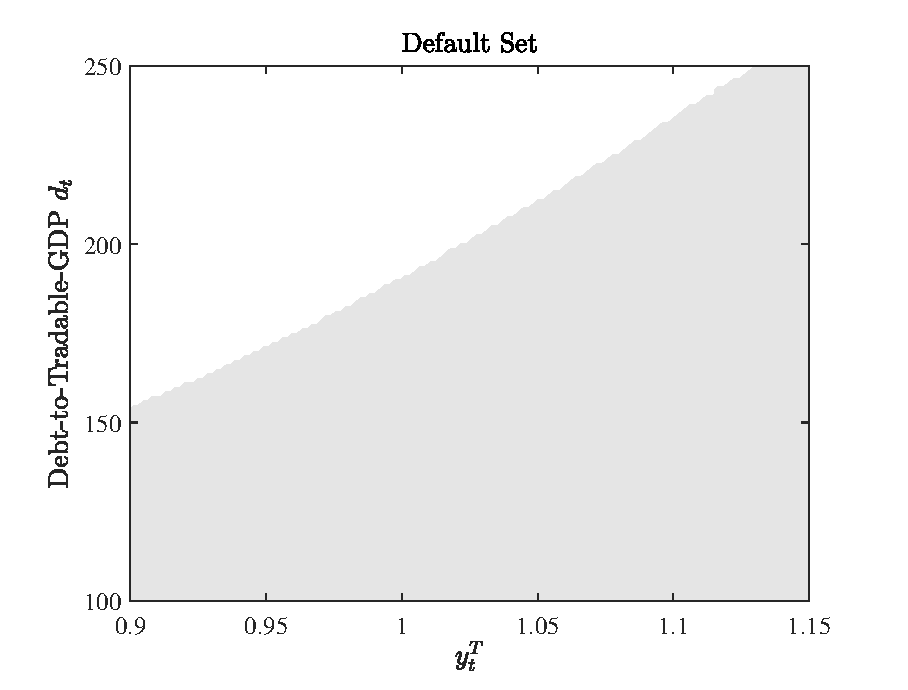
\includegraphics[height = 0.7\textheight]{fig/default_set_sri_trad_hp.eps}

    \end{frame}

    \begin{frame}
        \frametitle{Price of Debt}
        \begin{itemize}
            \item $\Pr(I_{t+1}=1 \mid I_{t}=1)$ is probability that next period output falls into default set
            \begin{equation}
                q(y^T_t, d_{t+1}) =
                \frac{1 - \Pr\left\{ y^T_{t+1} \in D(d_{t+1}) \mid y^T_t \right\}}{1 + r^*}
            \end{equation}
            \item Since $y^T_t$ is AR(1), output today is enough information about tomorrow $\rightarrow$ function of $y^T_t$
        \end{itemize}
    \end{frame}

    \begin{frame}
        \frametitle{Optimal Devaluation Rate}
        \begin{itemize}
            \item Optimal labor supply: $h_t = \bar{h}$ or full employment
            \item To ensure full employment, wage must be
                \begin{equation}
                    w_t = w^f(c^T_t) \equiv \frac{A_2(c^T_t, F(\bar{h}))}{A_1(c^T_t, F(\bar{h}))} F'(\bar{h})
                \end{equation}
            \item Because downward rigidity
                \begin{equation*}
                    \gamma \le \frac{W_t}{W_{t-1}} = \frac{w_t}{w_{t-1}} \frac{P^T_t}{P^T_{t-1}} = \epsilon \frac{w_t}{w_{t-1}}
                \end{equation*}
            \item Optimal devaluation rate is any $\epsilon_t$ such that
                \begin{equation}
                    \epsilon_t \ge \gamma \frac{w_{t-1}}{w^f(c^T_t)}
                \end{equation}
        \end{itemize}
    \end{frame}

    \section{Calibration}
    \begin{frame}
        \frametitle{Parameters needed to be calibrated}
        \begin{tabular}[t]{r l}
            Param. & Description \\
            \hline\\
            $\rho$     & Autocorrelation of output\\
            $\sigma_u$ & Standard deviation of output\\
            $r^*$      & Risk-free rate\\
            $\theta$   & Probability of reentry\\
            $\alpha$   & Labor share in nontradable goods sector\\
            $a$        & Share of tradable consumption\\
            $\xi$      & Intratemporal elasticity of substitution of consumptin\\
            $\sigma$   & 1/(intertemperal elasticity of substitution of consumption)\\
            $\gamma$   & Downward wage rigidity\\
            $\beta$    & Discount factor\\
            $\delta_1$ & Coefficient of the linear term in loss function\\
            $\delta_2$ & Coefficient of the quadratic term in loss function\\

            \end{tabular}
    \end{frame}

   \begin{frame}
    \frametitle{General procedure}
    \begin{itemize}
        \item $\rho, \sigma_u$:  Per capita tradable GDP $\rightarrow$ HP-filter $\rightarrow$ cyclical component $\rightarrow$ AR(1) estimation $\rightarrow \hat{\rho}, \hat{\sigma}_u$
        \begin{itemize}
            \item Since model period is quarter, data period is year
            \item $\rho = 1 - \frac{1 - \hat{\rho}}{4}$, $\sigma_u = \frac{\hat{\sigma}_u}{\sqrt{4}}$
        \end{itemize}
        \item $r^*$: US 3-month T-bill $\approx 4\%$ per year
        \item $\theta$: 1 / average years till reentry
        \item $\alpha$: Follow calibration of literature
        \item $a$: mean of tradable-to-GDP ratio over 2001 to 2022
        \item $\sigma, \xi$: Follow literature, set as (2, 0.5)
        \item $\beta, \delta_1$: match three equilibrium moment
        \begin{itemize}
            \item Quarterly unsecured debt-to-tradable-GDP ratio
            \item Default frequency per century
            \item Average output loss in bad standings (As check)
        \end{itemize}
        \item $\delta_2 = (1 - \delta_1) / (2\max(y^T_t))$ to ensure output monotonicity during autarky.
    \end{itemize}
   \end{frame}

   \begin{frame}[allowframebreaks]
    \frametitle{Output process}
        \begin{itemize}
            \item HP-filter with $\lambda = 100$ since annual data
            \item Tradable = agriculture + forestry + fishing + industry
        \end{itemize}

        \framebreak

        Sri Lanka\\
       {         \centering
        \begin{tabular}[pos]{rrrr}
        Filtering &
        $\rho$ &
        $\sigma$ &
        \begin{tabular}[c]{@{}r@{}}Unconditional \\ std\end{tabular} \\
        \midrule
        HP                   & 0.8922   & 0.0198   & 4.38\% \\
        \bottomrule
        \end{tabular}
       }
        \\[2em]
        Zambia\\
        {
            \centering
        \begin{tabular}[pos]{rrrr}
        Filtering &
        $\rho$ &
        $\sigma$ &
        \begin{tabular}[c]{@{}r@{}}Unconditional \\ std\end{tabular} \\
        \midrule
        HP                  & 0.6592   & 0.0278  & 3.69\%  \\
        \bottomrule
        \end{tabular}
        }

    \end{frame}


    \begin{frame}
        \frametitle{Sri Lanka}
        \centering
        \begin{tabular}{@{}lll@{}}
        % \begin{tabular}{@{}lp{0.6\textwidth}lp{0.3\textwidth}@{}}
        \toprule
        Parameter  & Value  & Source                                                                         \\
        \midrule
        $\rho$     & 0.8922  & Estimation of AR(1) on GDP\\
        $\sigma_u$ & 0.0198 & Estimation of AR(1) on GDP \\
        $r^*$      & 0.01 & U.S. 3-month treasury bill rate \\
        $\theta$   & 0.0385 & \citet*{Chatterjee-12}                                              \\
        $\alpha$   & 0.75   & \citet{Jegajeevan-Sri-Lanka-DSGE}                                                       \\
        $a$        & 0.4   & Share of tradable goods in GPD                  \\
        $\xi$      & 0.5   & \citet{Na-18}                             \\
        $\sigma$   & 2   & $1 / \xi$                                                                      \\
        $\gamma$   & 0.95   & \citet*{wage-rigidity-data}                  \\
        $\beta$    & 0.6959  &  Estimated                                                                              \\
        $\delta_1$ &  -0.5265 &   Estimated                                                                             \\
        $\delta_2$ &  0.6349   &   Set to ensure monotonicity                                                                 \\
        $\bar{h}$  & 1      & Normalized to 1\\
        \bottomrule
        \end{tabular}%

    \end{frame}

    \begin{frame}
        \frametitle{Zambia}
        \centering
        \begin{tabular}{@{}lll@{}}
        % \begin{tabular}{@{}lp{0.6\textwidth}lp{0.3\textwidth}@{}}
        \toprule
        Parameter  & Value  & Source                                                                         \\
        \midrule

        $\rho$     & 0.6592 & Estimation of AR(1) on GDP\\
        $\sigma_u$ & 0.0278 & Estimation of AR(1) on GDP\\
        $r^*$      & 0.01 & 3 month treasury bill rate \\
        $\theta$   & 0.0333 & \citet*{trebesch-2011-sovereign}                                              \\
        $\alpha$   & 0.66   &                                                        \\
        $a$        & 0.41   &Share of tradable goods in GDP                    \\
        $\xi$      & 0.5   & \citet{Na-18}                              \\
        $\sigma$   & 2   & $1 / \xi$                                                                      \\
        $\gamma$   & 0.87   & \citet*{wage-rigidity-data}                  \\
        $\beta$    & 0.6257  &  Estimated \\
        $\delta_1$ &  -0.6374 &   Estimated  \\
        $\delta_2$ &  0.7010   &     Set to ensure monotonicity   \\
        $\bar{h}$  & 1      & Normalized to 1\\
        \bottomrule
        \end{tabular}%
    \end{frame}

    \section{Result}

    \begin{frame}[label = {sri_ds}]
        \frametitle{Sri Lanka Default Set}
        \centering
        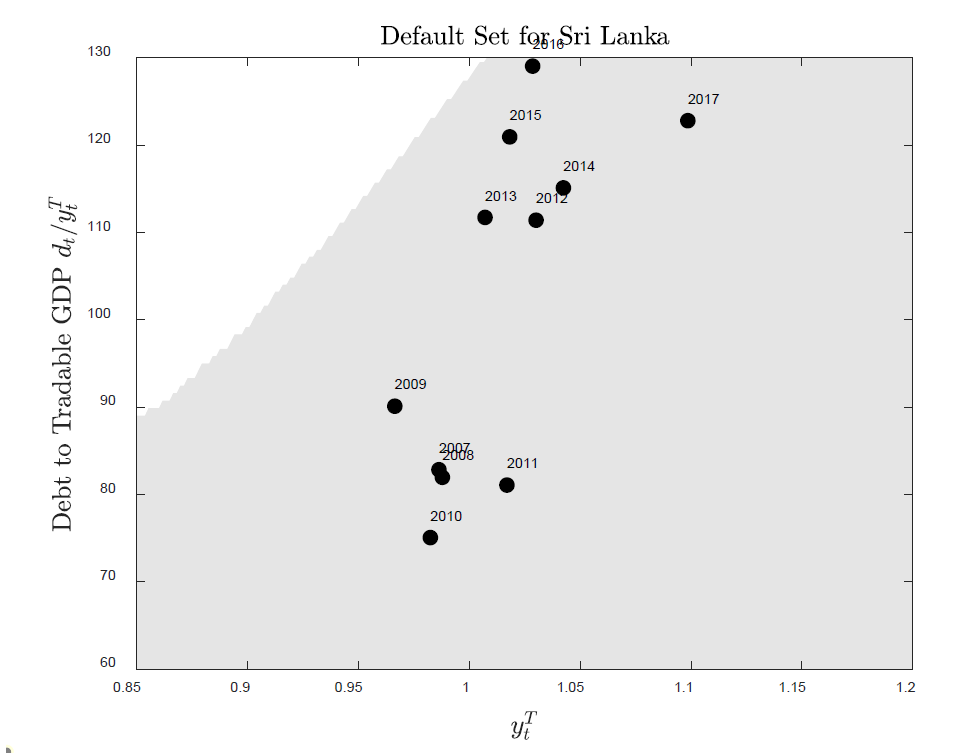
\includegraphics[width = 0.8 \textwidth]{fig/sri_with_china_v2.png}\\
    \end{frame}

    \begin{frame}[label = {pak_ds}]
        \frametitle{Zambia Default Set}
        \centering
        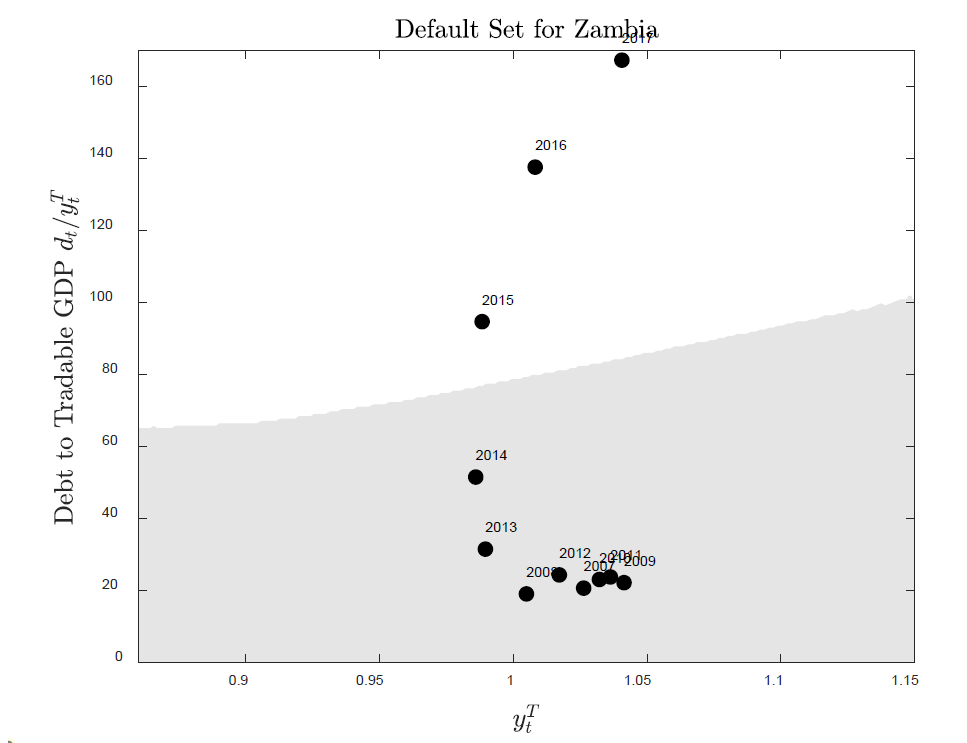
\includegraphics[width = 0.8 \textwidth]{fig/zam_with_china_v2.png}\\
    \end{frame}

    \begin{frame}
        \frametitle{Removing China's Debt}
        \centering
        \only<1-2>{Sri Lanka\\}
        \only<3-4>{Zambia\\}
        \includegraphics<1>[width = 0.8 \textwidth]{fig/sri_with_china_v2.png}%
        \includegraphics<2>[width = 0.8 \textwidth]{fig/sri_x_china_v2.png}%
        \includegraphics<3>[width = 0.8 \textwidth]{fig/zam_with_china_v2.png}%
        \includegraphics<4>[width = 0.8 \textwidth]{fig/zam_x_china_v2.png}%
    \end{frame}

    \begin{frame}
        \frametitle{Problems with Removing China's Debt}

        \begin{itemize}
            \item Debt is endogenous in the model --- Might borrow from other countries
            \begin{itemize}
                \item Hambantota Port is originally the former President's idea
                \item Pakistan is under severe power shortage, might borrow money for infrastructure constructions
            \end{itemize}
            \item GDP might be lower --- BRI investment might have cause the counties' GDP to grow
            \begin{itemize}
                \item BRI investment may increase labor demand on industrial sectors
            \end{itemize}
            \item Counterfactual analysis must account for the two factor.
        \end{itemize}

    \end{frame}

    \begin{frame}
        \frametitle{Is it all China to Blame?}
        \centering
        \includegraphics<1>[width = 0.8 \textwidth]{fig/sri_x_other.png}
        \includegraphics<2>[width = 0.8 \textwidth]{fig/zam_x_other.png}

    \end{frame}

    \begin{frame}
        \frametitle{Foreign Bonds as a Major Component}
        \citet{moramudali2022evolution}:
        \begin{itemize}
            \item Debt service on international sovereign bonds amounted to 47\% of Sri Lanka’s
government external debt servicing in 2021
        \item the share of Chinese debt was 20\%
        \end{itemize}

        \citet{brautigam2022zambia}:
        \begin{itemize}
            \item Nov 2022: Default on its foreign bonds
        \end{itemize}

    While much discussion on the debt trap thesis has focused on China, there are clearly other overlooked big fish in the debt pond.
    \end{frame}

    \appendix
    \begin{frame}[allowframebreaks]
            \frametitle{References}
            \bibliographystyle{econ}
            \bibliography{bib/ref}
    \end{frame}
\end{document}